\section{Discussion of Results}
Since PDF, i.e., input files of the NLP Engine architecture consist of unstructured text and for instance, undesired characters may remain despite text parsing, it is mandatory determine the \textit{accuracy} of the results obtained once the output JSON file has been populated. For this purpose, two types of experiments have been conducted to determine the \textit{accuracy} of the results. On the one hand, a simple inspection at sub-article level and on the other hand, a verification based on symbol comparison. The tests are performed on two Roaming Agreements sample of the MNOs Proximus and Orange \cite{proximus}. Each experiment is described below and the results obtained are discussed in the same section.

\subsection{Accuracy determination based on a simple inspection at sub-article level}
The first accuracy analysis consists of determining by simple inspection, i.e., human-eye inspection, whether each sub-article of the roaming agreement constitutes a \textit{variation}, a \textit{standard clause} or a \textit{customized text} with respect to the GSMA standard template. The results obtained are then compared with the values populated in the NLP Engine output file, for the same sub-article. Considering that the results obtained from the simple inspection constitute the observations and the values collected from sub-articles classification file constitute the predicted values, the following confusion matrices allow us to analyze the results for each sample roaming agreements. In this regard, the confusion matrix in the Table~\ref{table1} indicates that the \textit{accuracy} at which the 72 sub-articles analyzed are satisfactorily classified by the NLP Engine as \textit{standard clauses}, \textit{variations} or \textit{customized texts} is acceptable. Proof of this is the fact that the main diagonal of the matrix concentrates the highest number of True Positives. Table~\ref{table3} summarizes the accuracy of the NLP Engine's sub-article classification capability in percentage terms as \textit{standard clauses}, \textit{variations} and \textit{customized texts}.

\begin{table}[htbp]
\caption{Confusion Matrix for Proximus Roaming Agreement.}
\begin{center}
\begin{tabular}{|c|c|c|c|}
\hline
\textbf{n = 72} & \textbf{\textit{stdClause}}& \textbf{\textit{variation}}& \textbf{\textit{customText}} \\
\hline
\textbf{\textit{stdClause}}& 21 & 3 & 1 \\
\hline
\textbf{\textit{variation}}& 2 & 35 & 4 \\
\hline
\textbf{\textit{customText}}& 0 & 1 & 5 \\
\hline
\end{tabular}
\label{table1}
\end{center}
\end{table}

\begin{table}[htbp]
\caption{Confusion Matrix for Orange Roaming Agreement.}
\begin{center}
\begin{tabular}{|c|c|c|c|}
\hline
\textbf{n = 86} & \textbf{\textit{stdClause}}& \textbf{\textit{variation}}& \textbf{\textit{customText}} \\
\hline
\textbf{\textit{stdClause}}& 14 & 0 & 1 \\
\hline
\textbf{\textit{variation}}& 1 & 8 & 0 \\
\hline
\textbf{\textit{customText}}& 4 & 1 & 57 \\
\hline
\end{tabular}
\label{table2}
\end{center}
\end{table}

The Table~\ref{table2}, as well as Table~\ref{table1}, shows satisfactory results for the NLP Engine's predictive capability, i.e., regarding the \textit{accuracy} at which the NLP Engine classifies properly the sub-articles as \textit{standard clauses}, \textit{variations} or \textit{customized texts} for the Orange sample roaming agreement. Using the same evaluation criteria, it is observed how the main diagonal of the confusion matrix in Table~\ref{table2} concentrates the highest number of True Positive. Table~\ref{table3} also summarizes the accuracy of the NLP Engine's sub-article classification capability in percentage terms as \textit{standard clauses}, \textit{variations} and \textit{customized texts}.

\begin{table}[htbp]
\caption{Summary of accuracy determination for simple inspection at sub-article level.}
\begin{center}
\begin{tabular}{|c|c|c|c|}
\hline
\textbf{} & \textbf{\textit{Proximus}}& \textbf{\textit{Orange}} \\
\hline
\textbf{\textit{stdClause}}& 80.9\% & 92.9\% \\
\hline
\textbf{\textit{variation}}& 82.9\% & 87.5\% \\
\hline
\textbf{\textit{customText}}& 80.0\% & 91.2\% \\
\hline
\end{tabular}
\label{table3}
\end{center}
\end{table}

Beyond the fact that the results themselves can be considered as acceptable, the other behavior to be highlighted in Table~\ref{table3} is the greater classification capacity into \textit{standard clauses}, \textit{variations} and \textit{customized texts} of the NLP Engine in one document with respect to another.

\subsection{Accuracy determination based on symbol comparison}
The second accuracy analysis involves establishing a comparison between the sub-articles populated in the output file with respect to the sub-articles existing in the input file containing the Roaming Agreements. This comparison is performed at the symbol level, considering the order of appearance of each symbol. For that purpose, the text comparison tool Countwordsfree (\cite{countwordsfree}) is used manually copying sub-article by sub-article. For each sub-article is determined:

\begin{enumerate}
\item Common percentage of symbols between compared sub-articles.
\item Difference percentage of symbols between compared sub-articles.
\item Common symbols between compared sub-articles.
\item Difference symbols between compared sub-articles.
\end{enumerate}

\begin{figure}[htbp]
\centerline{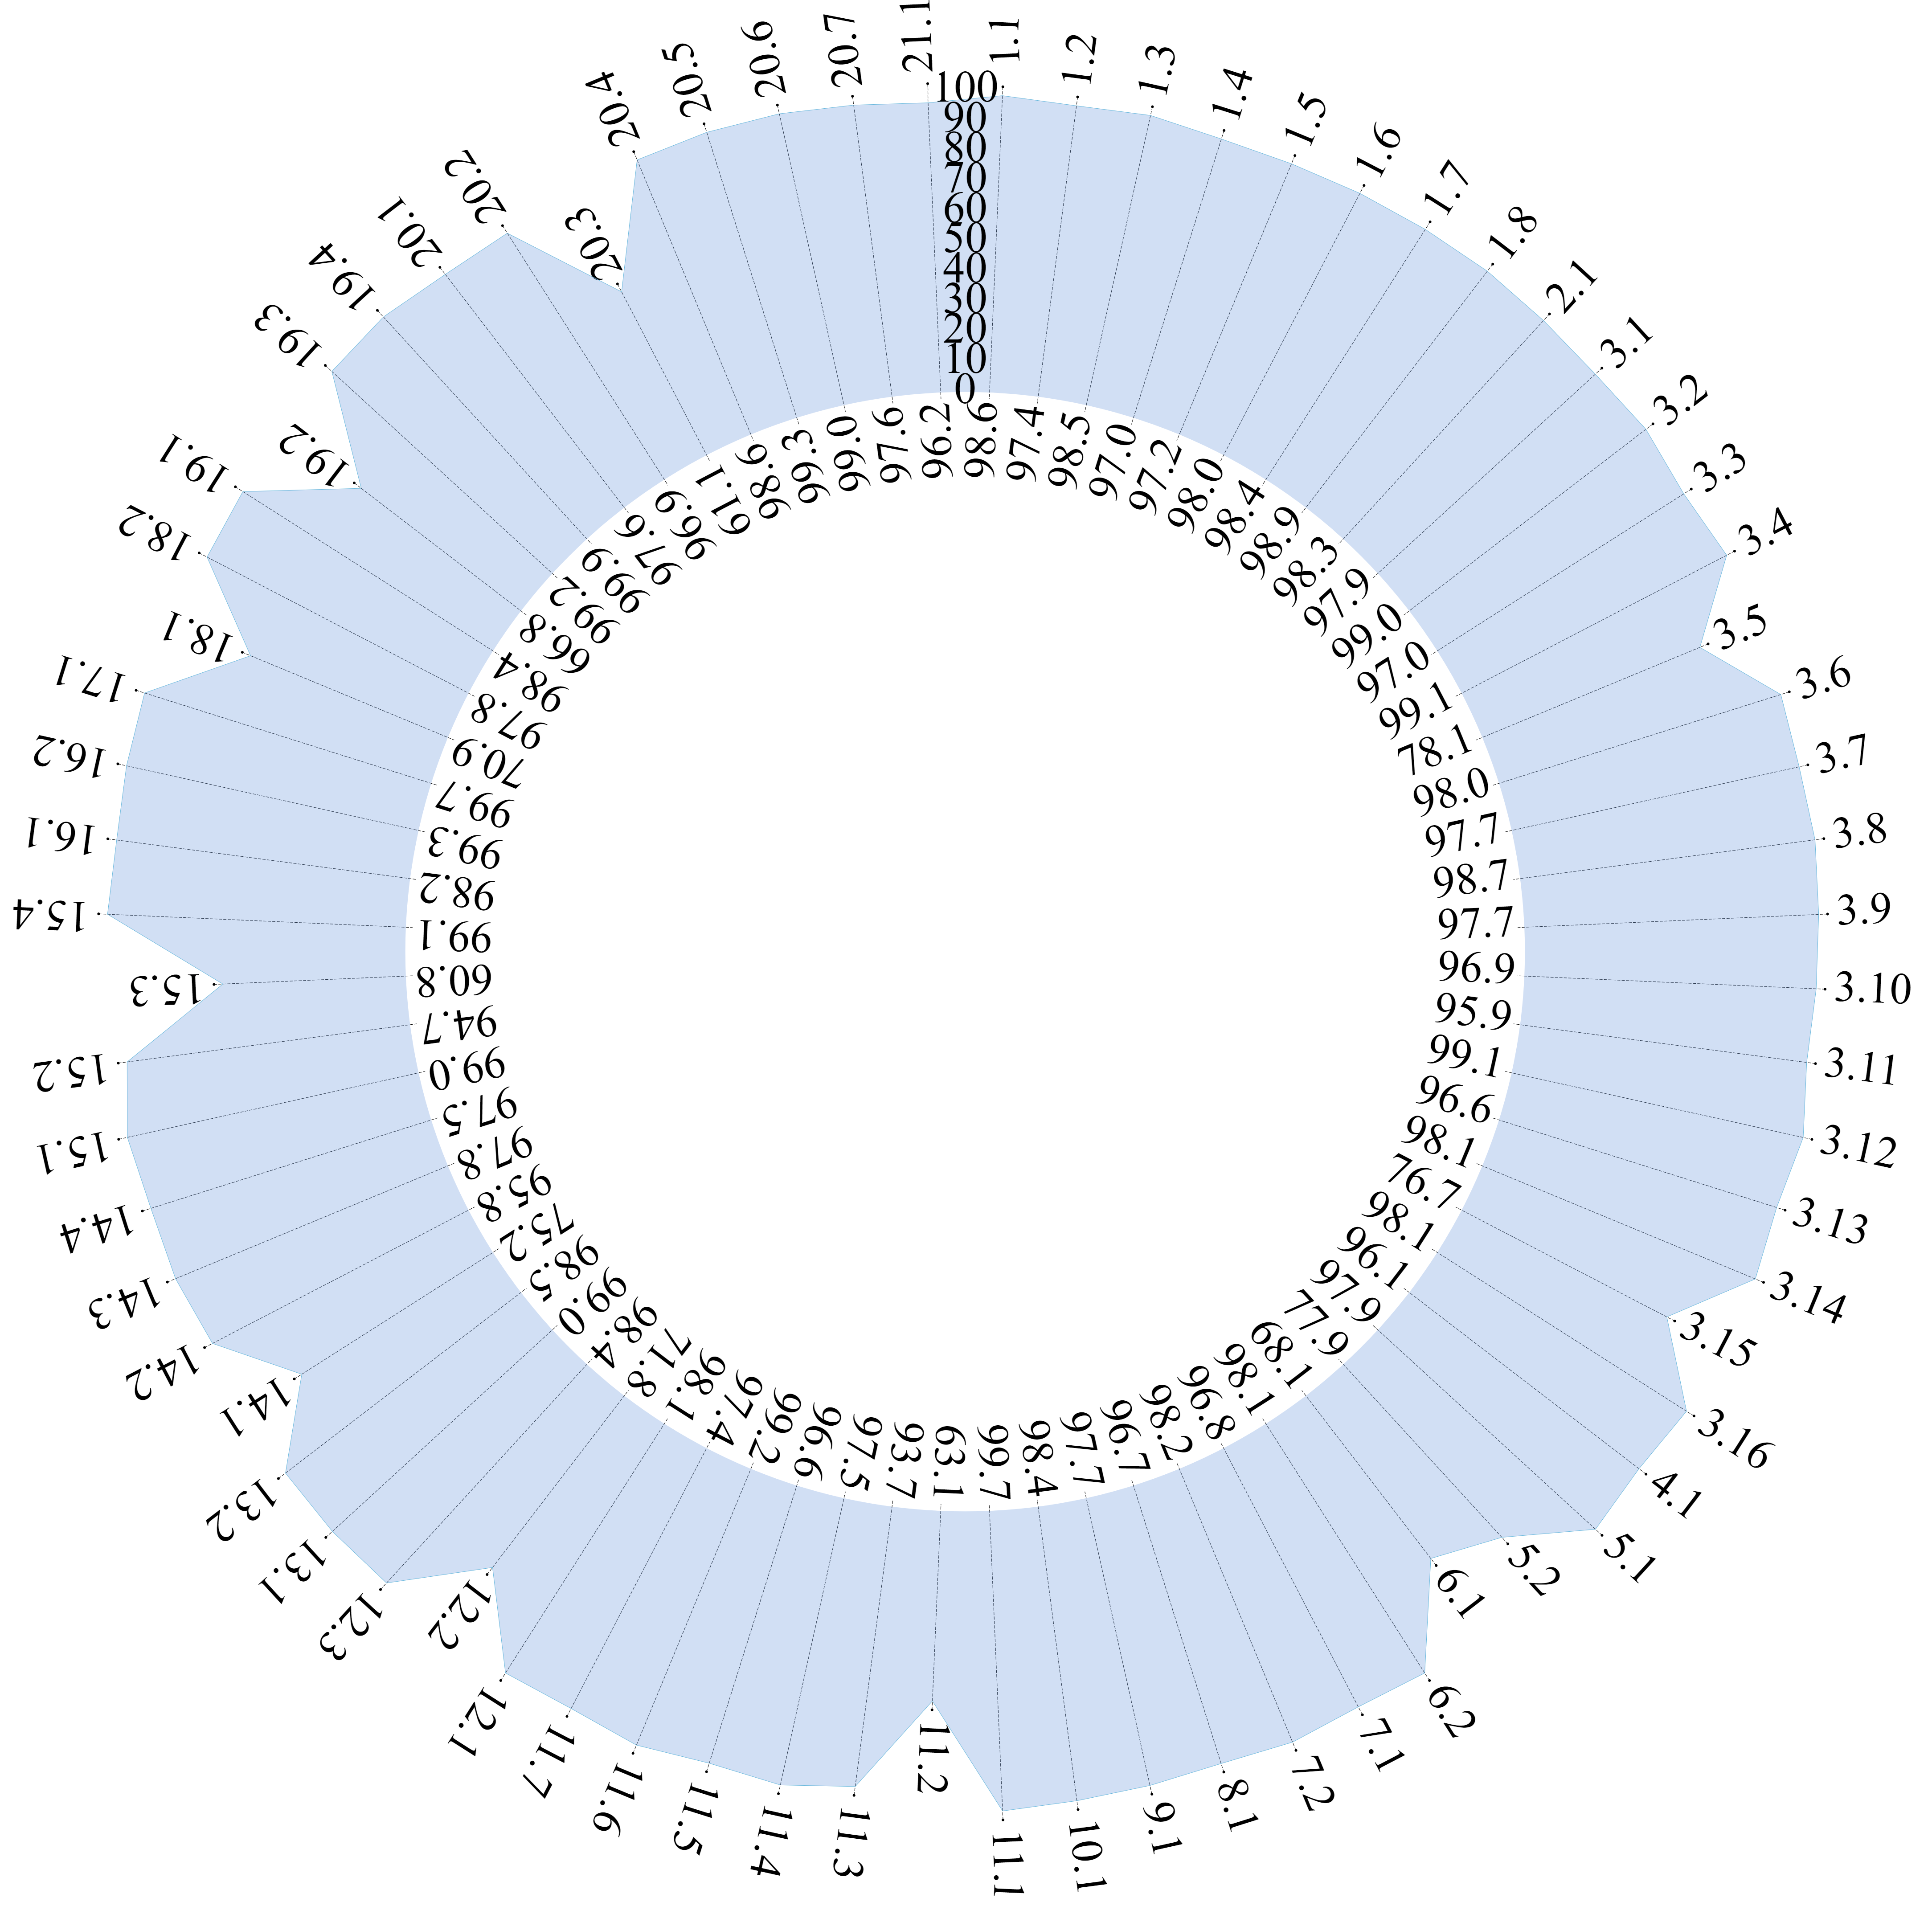
\includegraphics[width=0.43\textwidth]{images/Proximus.png}}
\caption{Common percentage of symbols for Proximus Roaming Agreement.}
\label{fig3}
\end{figure}

\begin{figure}[htbp]
\centerline{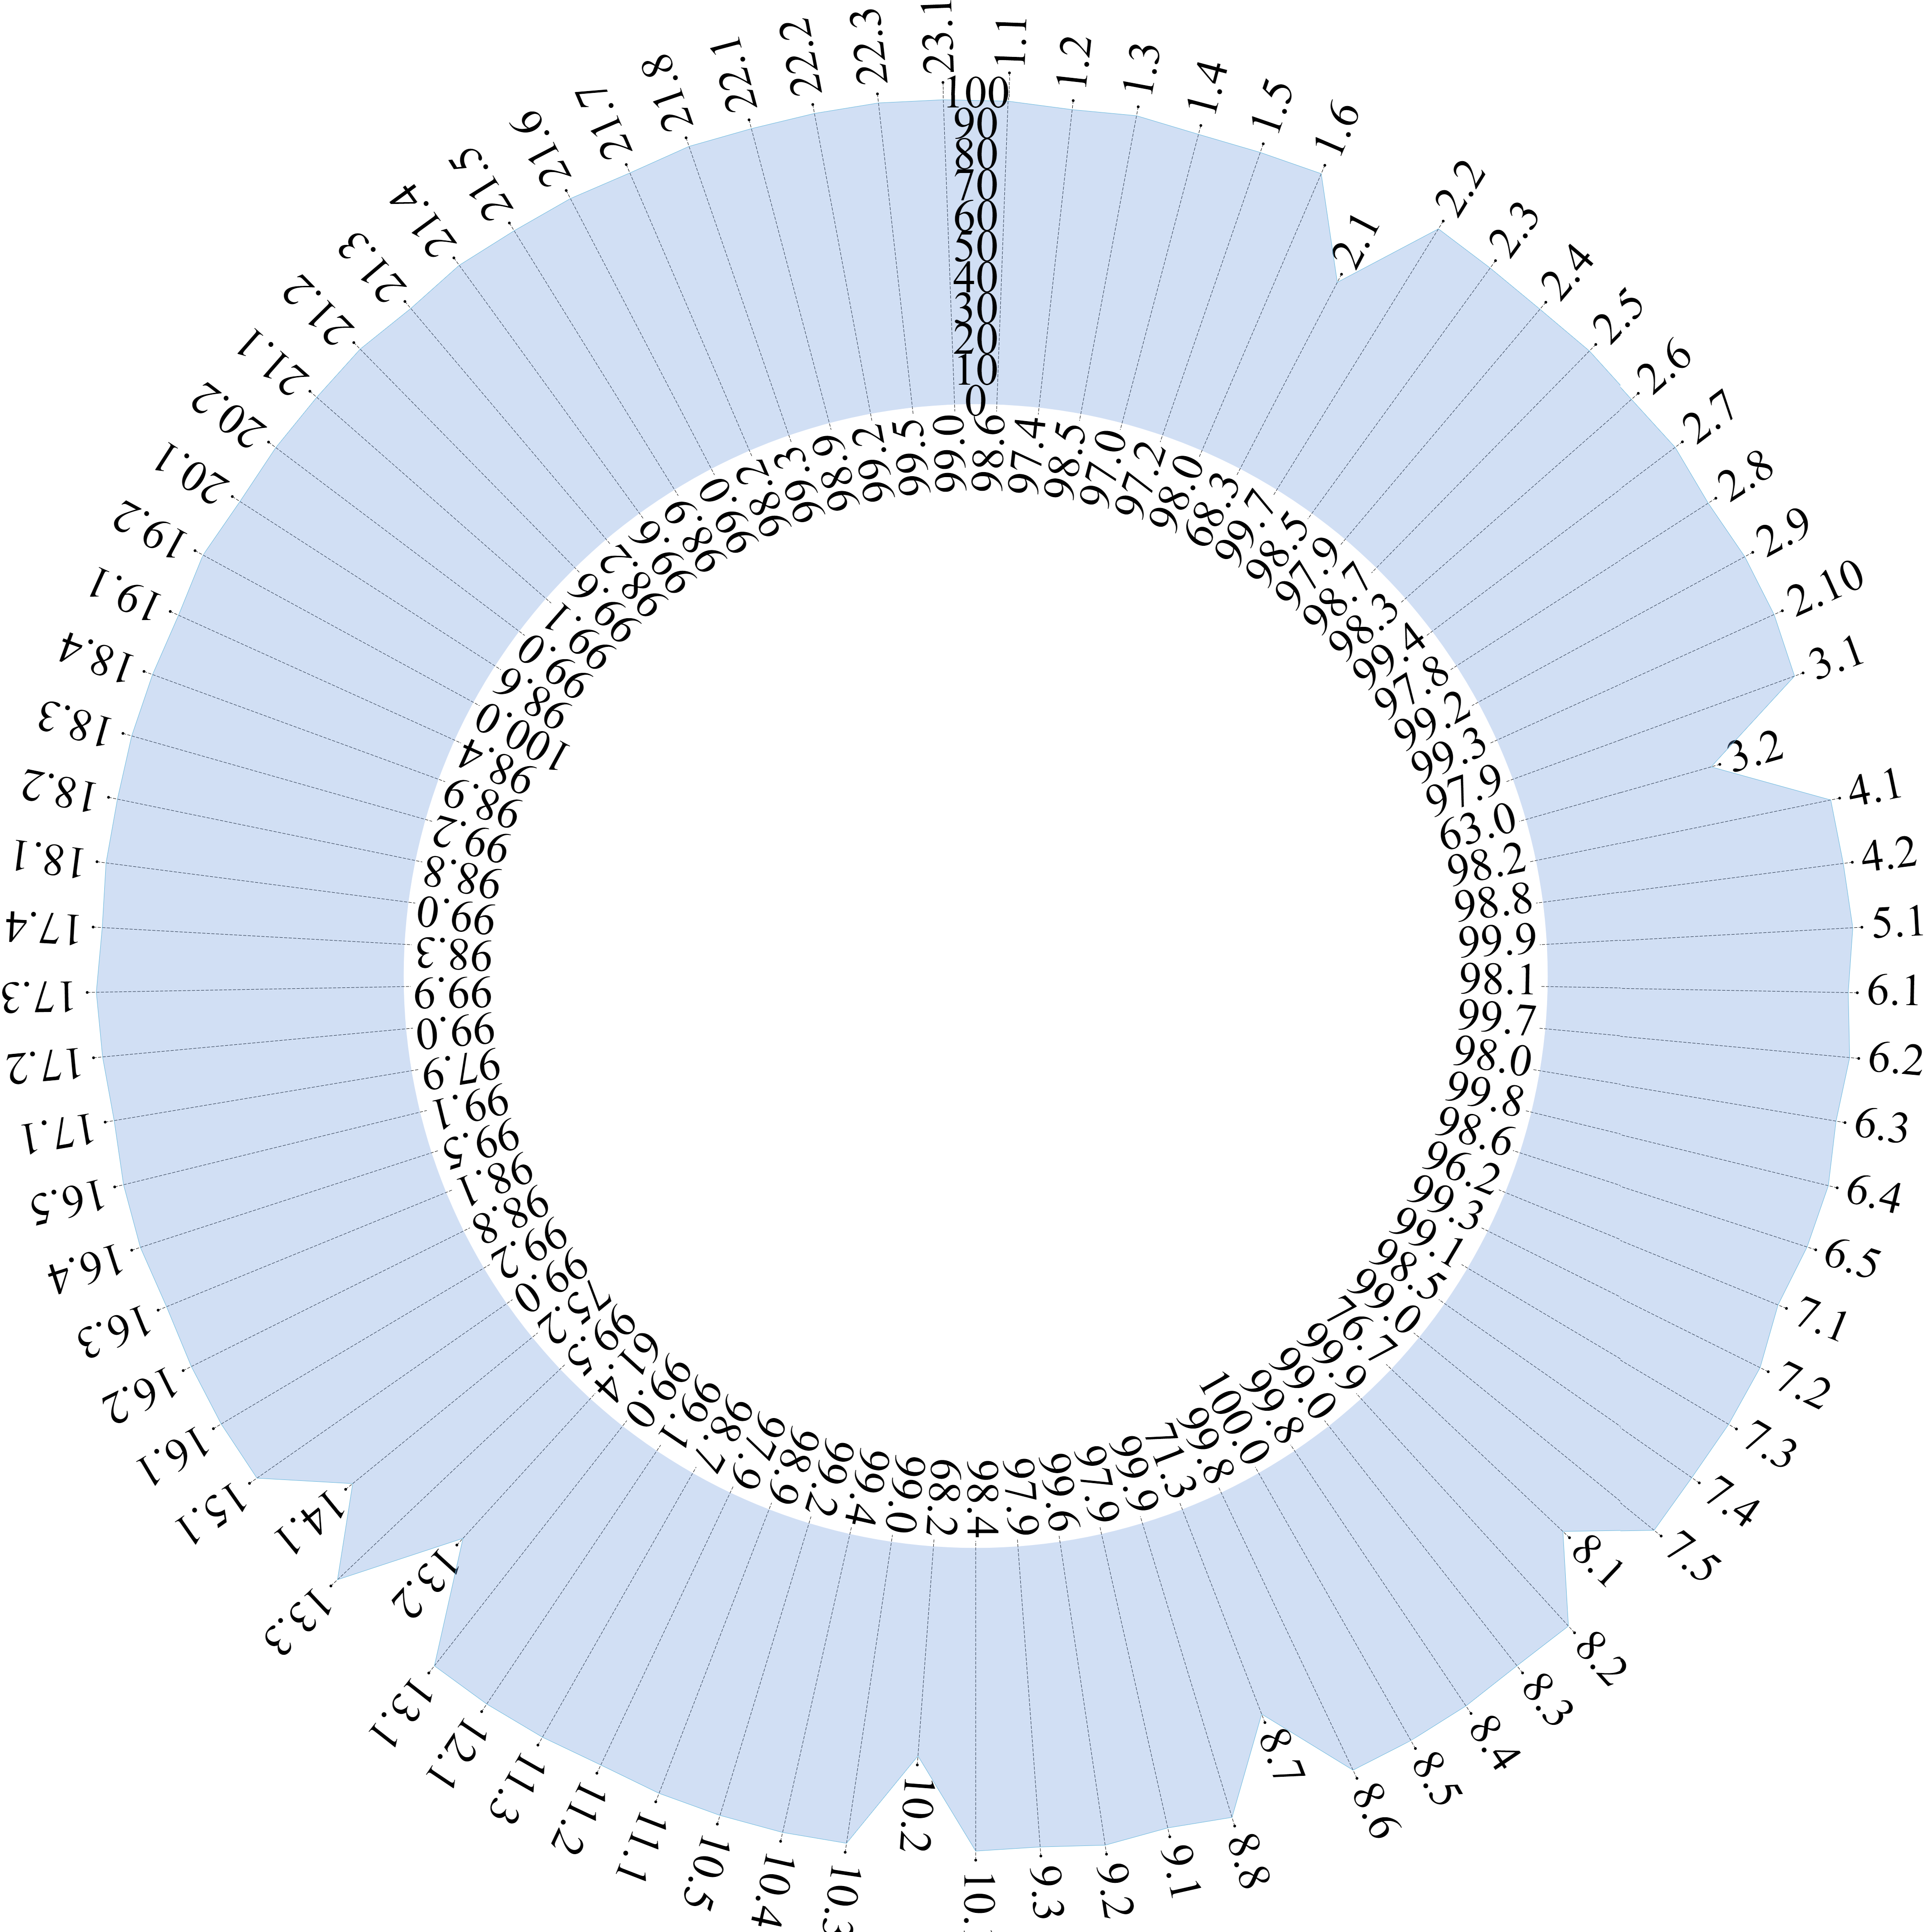
\includegraphics[width=0.43\textwidth]{images/Orange.png}}
\caption{NLP Engine overall architecture for Orange Roaming Agreement.}
\label{fig4}
\end{figure}

The following radar chart allow us to analyze the results for each roaming agreement. The radar chart contain in the inner radius the Common percentage of symbols between compared sub-articles and in the outer radius the identifier of the compared sub-article. Fig.~\ref{fig3} shows a comparison in terms of the common percentage of symbols between compared sub-articles for the Proximus sample roaming agreement. The conclusion that can be reached by simple inspection is that only 11 of the 72, i.e.,  84.7\% of the analyzed sub-articles are affected, mostly by the introduction of undesired characters when output file was populated.

Similarly, Fig.~\ref{fig4} shows a comparison in terms of the common percentage of symbols between the sub-articles compared for the Orange sample roaming agreement. In this case, only 7 of the 86, i.e., 91.9\% of the analyzed sub-articles are affected by the introduction of undesired characters when the output file is populated, thus improving the results obtained for the Proximus sample roaming agreement.
